%% ============================================================================
%% Manuscript prepared for: Journal of Survey Statistics and Methodology (JSSAM)
%% Following JSSAM Author Guidelines and ASA Style
%% ============================================================================

%% JSSAM accepts LaTeX with standard article class
%% Convert to PDF before submission
\documentclass[12pt]{article}

%% JSSAM formatting requirements: 1-inch margins, double-spacing, 12pt Times New Roman
\usepackage[margin=1in]{geometry}
\usepackage{setspace}
\doublespacing
\usepackage{times}  % Times New Roman font

%% Standard Packages
\usepackage{graphicx}
\usepackage{multirow}
\usepackage{amsmath,amssymb,amsfonts}
\usepackage{amsthm}
\usepackage{mathrsfs}
\usepackage[title]{appendix}
\usepackage{xcolor}
\usepackage{textcomp}
\usepackage{booktabs}
\usepackage{algorithm}
\usepackage{algorithmicx}
\usepackage{algpseudocode}
\usepackage{listings}
\usepackage{subcaption}

%% ASA-style citations (author-year format)
\usepackage[authoryear,round]{natbib}
\bibliographystyle{apalike}

%% For URLs in references
\usepackage{url}
\usepackage{hyperref}
\hypersetup{colorlinks=true,linkcolor=blue,citecolor=blue,urlcolor=blue}

%% Theorem styles
\theoremstyle{plain}
\newtheorem{theorem}{Theorem}
\newtheorem{proposition}[theorem]{Proposition}

\theoremstyle{definition}
\newtheorem{example}{Example}
\newtheorem{remark}{Remark}
\newtheorem{definition}{Definition}

\raggedbottom

\begin{document}

%% ============================================================================
%% TITLE PAGE (JSSAM requires word count on title page)
%% ============================================================================

\begin{center}
{\Large\bfseries Correction of Heaping at the Individual Level}

\vspace{1.5cm}

%% Author information removed for blind review
\textbf{[Author information removed for blind review]}

\vspace{1.5cm}

\textbf{Word count:} Approximately 6,500 words (excluding figures, tables, references, and appendices)

\vspace{0.5cm}

\textbf{Section:} Survey Statistics

\end{center}

\thispagestyle{empty}
\newpage

%% ============================================================================
%% ABSTRACT (max 300 words, non-technical language per JSSAM requirements)
%% ============================================================================

\begin{abstract}
\noindent
Heaping---the tendency to report values at round numbers---is a common phenomenon in survey data that can bias statistical analyses. Traditional correction methods smooth aggregated distributions but do not preserve individual-level data needed for regression modeling and longitudinal studies. This paper proposes a novel procedure for correcting heaping at the individual level by redistributing excess observations from heaped values using draws from truncated distributions (log-normal, normal, uniform, or kernel density estimates). A model-based variant incorporates covariate relationships to better preserve data structure. Simulation studies demonstrate that the proposed method effectively eliminates heaping, reducing Whipple index values from over 140 to approximately 100 (no heaping) and decreasing the mean absolute percentage error by up to 60\% compared to uncorrected data. Application to wage gap analysis using Blinder-Oaxaca decomposition shows that model-based correction achieves less than 2\% deviation from true coefficients, compared to over 10\% for naive correction. The methods are implemented in the R package \texttt{heaping}, providing accessible tools for researchers to correct heaping while maintaining individual-level data integrity for downstream analyses.

\vspace{0.5cm}
\noindent\textbf{Keywords:} heaping, age heaping, individual-level correction, truncated distributions, Whipple index, survey data quality
\end{abstract}

\vspace{1cm}

%% ============================================================================
%% STATEMENT OF SIGNIFICANCE (required by JSSAM, max 200 words)
%% ============================================================================

\noindent\textbf{Statement of Significance}

\vspace{0.3cm}

\noindent
Heaping---the clustering of reported values at round numbers---is pervasive in survey data collection, affecting variables such as age, income, weight, and time. While established methods exist to detect heaping through indices like Whipple's index, correction approaches have been limited to smoothing aggregated frequency distributions. This fundamentally restricts their utility: smoothed distributions cannot be used for individual-level analyses such as regression modeling, propensity score matching, or longitudinal record linkage. Our contribution addresses this gap by providing the first comprehensive framework for correcting heaping at the individual record level. The proposed method redistributes excess observations from heaped values to neighboring values using statistically principled approaches based on truncated distributions. A model-based variant preserves relationships between the heaped variable and covariates, which is critical for maintaining data integrity in multivariate analyses. The accompanying R package \texttt{heaping} makes these methods accessible to survey practitioners, enabling improved data quality for downstream statistical analyses while maintaining the individual-level structure that modern survey research requires.

\newpage

%% ============================================================================
%% MAIN TEXT
%% ============================================================================

\section{Introduction}\label{sec1}

\subsection{The Importance of Data Cleaning in Statistical Analysis}

Data cleaning is a crucial step in ensuring the quality and reliability of any statistical analysis. Real-world data sets often contain errors, missing values, and inconsistencies that can distort the results. A specific example is age heaping, where individuals tend to round their ages to numbers ending in 0 or 5, requiring correction to reflect accurate age distributions.

Clean data improves the accuracy of statistical models, leading to better predictions and more reliable outcomes. In data science, this process is formalized in methodologies such as CRISP-DM (Cross-Industry Standard Process for Data Mining), where data cleaning is a key part of the data preparation phase. This ensures that subsequent modeling is based on reliable data.


\subsection{Heaping in Data}

When the population age pyramid is not known for the surveyed population of interest, the age distribution still needs to be corrected to account for heaping effects. This is particularly relevant in survey data where the true underlying distribution cannot be directly observed \citep{ewbank1981}.

Heaping occurs when data values are disproportionately concentrated around certain points, typically due to rounding or preference for certain numbers. This phenomenon can appear in various types of data, whereby age heaping is often discussed in literature. Hereby, people often report ages ending in 0 or 5 more frequently than other ages. This can result from lack of precise age knowledge or rounding to familiar numbers. Another case is income heaping where individuals may round their income to the nearest thousand, ten thousand, or other significant figures, leading to peaks at these rounded values. In weight and height heaping people may round their weight or height to the nearest 5 or 10 units, causing concentrations at these values. There is also time heaping such as the duration of events or the timing of activities, that can exhibit heaping when people round to the nearest 5, 10, or 15 minutes. In some financial transactions, heaping may occur, when amounts in financial transactions (e.g. expenses, revenues) may show heaping at round figures (e.g. \$100, \$1,000).
And there is measurement data heaping when values may be rounded to the nearest convenient unit, causing heaping.

\subsection{Heaping Avoidance and Approaches to Deal with Heaping}

There are three solutions to the problem, and the first two might not always be possible to apply.

The first one is based on education and public awareness by improving respondents' understanding of the importance of accurate reporting can reduce heaping.

The second approach is based on methodological improvements by enhancing data collection methods, and training enumerators to avoid rounding can mitigate heaping effects.

The third approach---and content of this contribution---is the correction of heaping. By addressing the accumulation of various types of data, researchers and policy makers can ensure more reliable and valid conclusions, leading to better informed decisions and resource allocation.



\subsection{Reasons to Smooth Heaping Effects}

One aim at accurate statistics, e.g. accurate counts of school-aged children ensure proper resource allocation, income data accuracy is crucial for tax policies, social benefits, and economic planning, and precise age data inform public health initiatives and resource distribution.

Smoothing heaping effects is essential across different types of data to ensure accuracy and reliability.


\begin{itemize}
    \item
    Age heaping artificially distorts the age structure of a population, resulting in inaccurate population pyramids and indicators, and leading to erroneous conclusions about demographic patterns in the population \citep{un13}.
    Flawed age structures may also lead to inaccurate future population projections. Age data are used to calculate mortality, fertility, and other rates. Misreporting might bias these rates.
    \item Misreported incomes can affect economic studies, tax policy planning, and social welfare assessments \citep{seiver78}. Income heaping can skew economic models and forecasts, affecting policy decisions. Income data supports economic indicators such as poverty rates, inequality measures, and economic growth statistics. Reliable income data are essential for studying economic behavior and market dynamics.
    \item Accurate age and weight data are vital in epidemiological research to identify disease patterns and show lower predictive validity \citep{stavrakantonaki17}.
\end{itemize}







\subsection{Indices to Measure Heaping}

Heaping refers to the tendency of individuals to report numbers ending in specific digits.
For age heaping, several indices exist.
For example, DemoTools \citep{aburto2022} include the Whipple \citep{spoorenberg2007}, Myers \citep{myers1954}, Bachi \citep{bachi1951}, Coale-Li \citep{coale1991}, Noumbissi \citep{noumbissi1992}, Spoorenberg \citep{spoorenberg2007}, Jdanov \citep{jdanov2008}, and Kannisto \citep{kannisto1999} age-heaping indices. Although the exact interpretation of these indices may differ, they generally show a strong correlation when applied to the same data and age ranges \citep{aburto2022}. Therefore, for quickly assessing the level of heaping across a large dataset, it may not be necessary to use more than one or two indices \citep{aburto2022}.

All of these indices are also implemented in the \texttt{heaping} R package introduced in this paper. The package provides the functions \texttt{whipple()} (standard and modified), \texttt{myers()}, \texttt{bachi()}, \texttt{noumbissi()}, \texttt{spoorenberg()}, \texttt{coale\_li()}, \texttt{jdanov()}, and \texttt{kannisto()}, as well as a convenience function \texttt{heaping\_indices()} that calculates all indices simultaneously. All functions support sample weights, making them suitable for survey data analysis. Additionally, the \texttt{sprague()} function implements the Sprague multipliers \citep{sprague1880} for disaggregating five-year age groups into single-year ages.

The most commonly used \citep{rasul23} and simplest to compute index is the original Whipple's index
proposed by George Chandler Whipple (1866-1924). It is a well-established index for detecting and analyzing age heaping.
The Whipple Index quantifies the extent of age heaping by comparing the reported frequencies of ages ending in 0 and 5 to those ending in other digits. It is calculated for a specific age range, typically 23 to 62 years.

Let \( P(a) \) represent the observed population at age \( a \). The Whipple Index \( W \) for the age range \( a = 23 \) to \( a = 62 \) is defined as:

\[
W = \frac{\sum_{a \in \{25,30,35,40,45,50,55,60\}} P(a)}{\frac{1}{5} \sum_{a=23}^{62} P(a)} \times 100
\]

The numerator sums the populations at all ages ending in 0 or 5 within the
range (eight ages: 25, 30, 35, 40, 45, 50, 55, 60).
The denominator represents the expected count at these ages under
a uniform distribution. Since the range 23--62 contains 40 single-year ages,
and 8 of these end in 0 or 5, we expect $8/40 = 1/5$ of the total
population to fall on these ages if there is no heaping.
Thus, dividing by $\frac{1}{5} \sum_{a=23}^{62} P(a)$ gives the
expected count, and the ratio (multiplied by 100) yields an index
where $W = 100$ indicates no heaping, reflecting an accurate age distribution \citep{un55}.
Values between 100 and 105 indicate very slight heaping, which is almost negligible. When the index is between 105 and 110, it suggests slight heaping that remains acceptable for high-quality data. Moderate heaping, represented by values between 110 and 125, shows a noticeable age rounding that could affect demographic analyzes. Strong heaping, indicated by an index between 125 and 175, signifies significant distortions, requiring cautious use of the data. Values above 175 reveal very strong heaping, rendering the data highly unreliable for demographic studies. See further details in \citet{shryock76}.



\subsection{Approaches to Correcting Heaping in Data}

Heaping, the disproportionate concentration of data values around specific points, is a common issue across various types of data, including age, income, weight, and financial transactions.
The simplest way to analyze age-heaping is by assuming that the true numbers are rectangularly distributed over some age range that includes centered the age in question \citep{hobbs2004}.



Correcting heaping is essential to ensure the accuracy and reliability of data analyses.



There are two principal methods for addressing heaping: correcting aggregated statistics and correcting individual values. Each method has its distinct advantages and applications.

\subsubsection{Correcting Aggregated Statistics}

The traditional approach to smoothing heaping effects
involves correcting aggregated statistics
such as age (histogram-like) distributions,
population pyramids, or income (histogram)
distributions.
This method is particularly useful for high-level demographic and economic analyses
where individual data points are not as critical.

Statistical techniques like moving averages, kernel density estimation, or spline smoothing can be applied to smooth out observed distributions. For example, in demographic studies, adjustment factors derived from historical data or known demographic patterns can redistribute heaped counts across a plausible range of values. This approach ensures that the overall distribution follows expected patterns, which is crucial for reporting and policy-making.

The simplicity and ease of implementation are significant advantages of this method.
It is suitable for large-scale analyses where the focus is on aggregated data trends.
However, this method may introduce bias if the adjustment factors or smoothing techniques
not appropriately chosen. Additionally, it does not correct individual records,
which can be problematic for further detailed analyses or modeling using non-aggregated data.

\subsubsection{Correcting Individual Values}

A more granular approach involves correcting the individual data points in a dataset to produce a smoothed aggregated statistic. This method, although more complex, provides precise corrections at the individual level, making it ideal for detailed analyses and modeling.

Model-based corrections use statistical models to estimate true values based on observed data. Bayesian methods or maximum likelihood estimation can infer the most probable true values. Simulation methods can also be employed, where corrected values are generated using distributions fitted to the non-heaped data, such as truncated normal or log-normal distributions. An alternative approach uses kernel density estimation to model the underlying distribution and correct for heaping \citep{kernelheaping}. Related methods for handling heaping effects in population data are also available in simulation packages such as simPop \citep{simpop}.

This approach ensures that individual-level data are accurate, allowing for comprehensive analyses such as longitudinal studies, regression analysis, and other detailed examinations. The primary advantage of this method is its precision and flexibility, as the corrected data can be utilized for various tasks. However, it requires more sophisticated statistical techniques and computational resources, and its accuracy depends heavily on the quality and amount of data available.

\subsubsection{Discussion}

Both approaches---correcting aggregated statistics and correcting individual values---offer unique advantages and are suitable for different contexts. The choice of method depends on the specific needs of the analysis, the available data, and the computational resources. While aggregated corrections are simpler and more suitable for high-level analyses, individual corrections provide the precision needed for detailed studies and modeling.

Smoothing heaping in data can be approached by either adjusting aggregated counts or changing individual observational values. The latter method, though more complex, offers several significant advantages:

\begin{enumerate}
\item Enhanced Data Accuracy for Individual-Level Analysis:
   The correction of individual values ensures that each data point reflects a more accurate measure. This precision is crucial for individual-level analyses, such as regression modeling, longitudinal studies, and other statistical analyses that require accurate input data. For example, when ages are corrected individually, the resultant data set better represents the true age distribution, leading to more reliable outcomes in studies that use age as a predictor or outcome variable.
\item Improved Flexibility in Data Usage:
   The correction of individual data can be used across various analyses without the need for repeated smoothing of aggregated data. This flexibility is particularly beneficial in demographic research, where the same data set can be used for multiple purposes, such as calculating age-specific fertility rates, mortality rates, and other demographic indicators. Users can apply the corrected data directly in their models, ensuring consistency across different analyses and reducing the risk of introducing errors through repeated data manipulation.
\item Better Detection and Correction of Anomalies:
   The adjustment of individual values allows for the identification and correction of specific anomalies in the data set, which might be obscured when only aggregated data is smoothed. This detailed approach can uncover patterns and trends that are not apparent in aggregated data. For instance, correcting individual income values in a survey data set can reveal more accurate distributions of income inequality and poverty, which are critical for policy-making and economic research.
\item Preservation of Data Granularity:
   Individual-level correction maintains the granularity of the data, which is essential for detailed analysis. Aggregated smoothing methods can sometimes mask important variations within the data, leading to the loss of valuable information. Furthermore, detailed demographic studies, such as those that examine the effects of age-specific policies, benefit significantly from granular data that accurately reflect individual variations.
\item Enhanced Data Integrity for Machine Learning Applications:
   In machine learning and predictive modeling, the quality of the input data directly impacts the performance of the models. Correcting individual values ensures that the data fed into the models is accurate and reliable, leading to better model training and more robust predictions. For example, age or income data corrected at the individual level can improve the performance of predictive models in healthcare, finance, and social sciences.
\item Consistency in Longitudinal Studies:
   Longitudinal studies that track individuals over time require consistent and accurate data at each time point. Correcting individual values ensures that longitudinal data remain accurate throughout the study period, enhancing the validity of the study findings. This approach is particularly important in studies examining changes over time, such as aging studies, where precise age data is critical.
\end{enumerate}


Although smoothing aggregated counts can provide a quick fix for age heaping, adjusting individual observational values offers more precise, flexible, and reliable data for a wide range of analyses. This method preserves data granularity, enhances the accuracy of individual-level analyses, and improves the overall integrity of the data set, making it the preferred approach in many practical and research applications.


Smoothing of aggregated statistics assumes age misreporting, not underreporting. If there is age/sex-specific underreporting, smoothing inappropriately spreads it out \citep{preston1999}.




\subsection{Traditional Smoothing Methods for Aggregated Data}

Several classical methods exist for smoothing age heaping in aggregated frequency data. These methods operate on age-specific counts $N(a)$ and produce smoothed counts $N'(a)$ by computing weighted averages of neighboring age frequencies. The most widely used approaches include:

\begin{itemize}
    \item \textbf{Carrier-Farrag} \citep{carrier1959}: Simple three-point moving average using immediate neighbors.
    \item \textbf{Arriaga} \citep{arriaga1968}: Five-point weighted average with decreasing weights for more distant ages.
    \item \textbf{Karup-King-Newton} \citep{karup1903}: Five-point formula with binomial-like weights (1:4:6:4:1).
    \item \textbf{United Nations} \citep{un1956}: Five-point formula with weights (1:2:3:2:1), designed to preserve population totals.
\end{itemize}

All these methods share common characteristics: they are computationally simple, assume approximately uniform age distributions within the smoothing window, and---most importantly---they correct \emph{aggregated frequency counts} rather than individual observations. While effective for producing smoothed population pyramids and demographic indicators, they cannot be applied when individual-level data are needed for regression analysis, longitudinal studies, or machine learning applications.

A more sophisticated approach is kernel density estimation for heaped data \citep{kernelheaping}, which estimates a smooth probability density function accounting for the heaping pattern. While this method provides improved distributional estimates compared to simple moving averages, it still operates at the aggregate level and produces density estimates rather than corrected individual records.


\subsection{Comparison of Correction Approaches}

All methods discussed above---Carrier-Farrag, Arriaga, Karup-King-Newton, and
United Nations---operate on \emph{aggregated data}, specifically on frequency counts $N(a)$ at each age $a$. They produce smoothed frequency distributions $N'(a)$ but do not modify individual records. Similarly, the kernel density estimation approach for heaped data \citep{kernelheaping} estimates a smooth probability density function from heaped observations, providing improved distributional estimates but not corrected individual values.

Table~\ref{tab:comparison} summarizes the key differences between these aggregated approaches and the individual-level correction method proposed in this paper.

\begin{table}[!htp]
\caption{Comparison of heaping correction approaches}\label{tab:comparison}
\centering
\begin{tabular}{lcc}
\toprule
\textbf{Characteristic} & \textbf{Aggregated Methods} & \textbf{Individual-Level} \\
\midrule
Input & Frequency counts $N(a)$ & Individual values $x_i$ \\
Output & Smoothed counts $N'(a)$ & Corrected values $x'_i$ \\
Preserves sample size & Yes (totals) & Yes (records) \\
Preserves individual records & No & Yes \\
Suitable for regression & No & Yes \\
Suitable for longitudinal analysis & No & Yes \\
Suitable for subgroup analysis & Limited & Yes \\
Suitable for machine learning & No & Yes \\
Uncertainty quantification & No & Yes (via multiple imputation) \\
\bottomrule
\end{tabular}
\end{table}

The aggregated methods are well-suited for producing accurate population pyramids, demographic indicators, and mortality/fertility rate calculations where only distributional summaries are needed. However, they cannot be used when:

\begin{itemize}
    \item Individual-level regression analysis is required (e.g., age as a predictor variable)
    \item Longitudinal studies track individuals over time
    \item Subgroup analyses require corrected individual records
    \item Machine learning models use age as a feature
    \item The corrected data must be linked back to other individual-level variables
\end{itemize}

The kernel density approach \citep{kernelheaping} provides a more sophisticated treatment of the heaping problem by estimating the underlying continuous distribution, but it still produces density estimates rather than corrected individual values. It is particularly useful for visualization and for understanding the true shape of the age distribution, but shares the same limitations as other aggregated methods when individual-level analysis is required.

The individual-level correction method proposed in this paper addresses these limitations by modifying a proportion of heaped values directly, preserving the data structure for downstream analyses while removing the heaping artifact. Furthermore, by using random sampling and supporting a seed parameter, repeated applications of the correction can be used in a multiple imputation framework to properly account for correction uncertainty in subsequent statistical analyses.


\section{Correction of Heaping at Individual Level}

Let $x = (x_1, x_2, \ldots, x_n)$ denote a numeric vector of $n$ individual age
observations, where each $x_i \in \mathbb{R}_{\geq 0}$ represents the reported
age of the $i$-th individual in the dataset. Due to heaping, certain values in $x$---typically those ending in 0 or 5---occur more frequently than expected under a smooth age distribution. The goal is to produce a corrected vector $x' = (x'_1, x'_2, \ldots, x'_n)$ of the same length, where a proportion of the heaped values have been replaced with plausible alternatives drawn from a fitted distribution, while non-heaped values remain unchanged.

Algorithm~\ref{alg:correctHeaps} describes the main correction procedure, which orchestrates the overall process: handling missing values, generating heap intervals, fitting distributions, and iterating over each heap position. For each heap where correction is needed, Algorithm~\ref{alg:correctSingleHeap} performs the actual replacement of values. This modular design mirrors the implementation in the \texttt{heaping} R package, where \texttt{correctHeaps()} handles the orchestration and calls internal functions for individual heap corrections.

The key input parameters are: the heaping pattern \texttt{heaps} (specifying whether heaping occurs at 5-year or 10-year intervals, or at custom positions), the distribution \texttt{method} used for generating replacement values, and an optional \texttt{seed} for reproducibility. Additionally, a \texttt{model} formula and associated \texttt{dataModel} can be provided to enable model-based sign adjustment, which uses covariate information to determine the direction of corrections.

\small

\begin{algorithm}
\small
\caption{Correct Heaping (Main Procedure)}\label{alg:correctHeaps}
\begin{algorithmic}[1]
\Require $x$ (ages), $heaps$ (``5year'', ``10year'', or numeric), $method$, $start$, $fixed$, $seed$, $model$, $dataModel$
\Ensure Corrected vector $x'$

\If{$seed$ provided} set random seed \EndIf
\State Handle NA values: store indices $na\_idx$, work with $x_{work} \gets x[\text{non-NA}]$

\State \textbf{// Generate heap intervals}
\If{$heaps$ is character}
    \State $step \gets 5$ if ``5year'', else $10$; \quad $intervals \gets \{start, start{+}step, \ldots, \max(x_{work})\}$
\Else
    \State $intervals \gets heaps$ (custom positions)
\EndIf

\State \textbf{// Calculate heaping ratios}
\State $counts \gets$ frequency table of $x_{work}$
\For{each $s$ in $intervals$}
    \State $ratio[s] \gets counts[s] \,/\, \text{mean}(counts[s{-}1], counts[s{+}1])$
\EndFor

\State \textbf{// Fit distribution parameters}
\State $params \gets$ fit distribution to $x_{work}$ based on $method$

\State \textbf{// Optional: fit prediction model}
\If{$model$ provided}
    \State $\hat{x} \gets$ random forest predictions from $dataModel$
\EndIf

\State $x_{orig} \gets x_{work}$
\For{each $s$ in $intervals$ where $ratio[s] > 1$}
    \State $x_{work} \gets$ \Call{CorrectSingleHeap}{$x_{work}, s, ratio[s], heaps, method, params, fixed$}
\EndFor

\State \textbf{// Model-based sign adjustment (if model provided)}
\For{each $i$ where $x_{work}[i] \neq x_{orig}[i]$}
    \If{$\text{sign}(x_{work}[i] - x_{orig}[i]) \neq \text{sign}(\hat{x}[i] - x_{orig}[i])$}
        \State $x_{work}[i] \gets x_{orig}[i] - (x_{work}[i] - x_{orig}[i])$ \Comment{flip direction}
    \EndIf
\EndFor

\State Restore NA values at $na\_idx$
\State \Return $x_{work}$
\end{algorithmic}
\end{algorithm}

\begin{algorithm}
\small
\caption{Correct Single Heap}\label{alg:correctSingleHeap}
\begin{algorithmic}[1]
\Require $x$ (ages), $s$ (heap age), $ratio$, $heaps$ (type), $method$, $params$, $fixed$
\Ensure Updated vector $x$ with heap at $s$ corrected

\State $indices \gets$ positions where $x = s$
\State $n_{correct} \gets \lceil |indices| - |indices| / ratio \rceil$
\State $candidates \gets indices$ excluding $fixed$

\If{$|candidates| = 0$} \Return $x$ \EndIf
\State $n_{correct} \gets \min(n_{correct}, |candidates|)$

\State \textbf{// Define bounds and draw replacements}
\If{$heaps$ = ``5year'' or custom}
    \State $bounds \gets [s - 2, s + 2]$
    \State $selected \gets$ random sample of $n_{correct}$ from $candidates$
    \State $x[selected] \gets$ \Call{DrawFromTruncated}{$method, params, s, bounds$}
\ElsIf{$heaps$ = ``10year''}
    \State $n_1 \gets \lceil n_{correct} / 2 \rceil$, \quad $n_2 \gets n_{correct} - n_1$
    \State $selected_1 \gets$ sample $n_1$ from $candidates$
    \State $x[selected_1] \gets$ \Call{DrawFromTruncated}{$method, params, s, [s{-}4, s{+}4]$}
    \State $selected_2 \gets$ sample $n_2$ from remaining $candidates$
    \State $x[selected_2] \gets$ \Call{DrawFromTruncated}{$method, params, s, [s{-}5, s{+}5]$}
\EndIf

\State \Return $x$
\end{algorithmic}
\end{algorithm}

\normalsize

The \textsc{DrawFromTruncated} procedure generates replacement values from a truncated distribution (log-normal, normal, uniform, or kernel density) within the specified bounds, centered at the heap age $s$. Values are rounded to integers to maintain the discrete nature of reported ages.


\subsection{Interval Generation}

The \emph{intervals} define the age values at which heaping is assumed to occur---these are the candidate ages whose frequencies will be examined and potentially corrected. The interval sequence is determined by the \texttt{heaps} parameter and the \texttt{start} value.

For the common case of 5-year heaping (ages ending in 0 or 5), with the default $start = 0$:
\[
\text{intervals} = \{0, 5, 10, 15, 20, 25, \ldots, \max(x)\}
\]

For 10-year heaping (ages ending in 0 only), with $start = 0$:
\[
\text{intervals} = \{0, 10, 20, 30, \ldots, \max(x)\}
\]

The \texttt{start} parameter allows flexibility for non-standard heaping patterns. For example, if heaping occurs at ages 2, 12, 22, 32, \ldots (perhaps due to a specific survey design), setting $start = 2$ with 10-year intervals would capture this pattern. Alternatively, a custom numeric vector can be supplied directly to specify arbitrary heap positions (e.g., $\{18, 21, 30, 40, 50, 65\}$ for retirement-age studies).

\subsection{Count and Ratio Calculation}

Before correcting any values, Algorithm~\ref{alg:correctHeaps} must determine \emph{which} heap ages exhibit excess frequency and \emph{how many} observations should be corrected at each. This is accomplished by calculating a heaping ratio for each interval, which compares the observed count at a heap age to the expected count based on neighboring ages (lines 8--12 in Algorithm~\ref{alg:correctHeaps}).

The first step is to construct a frequency table of all ages in the dataset. For each age $k$ in the range $[0, \max(x)]$, we count how many observations take that value:
\[
\text{counts}(k) = \sum_{i=1}^{n} \mathbb{I}(x_i = k)
\]
where $\mathbb{I}$ is the indicator function that equals 1 when the condition is true and 0 otherwise, and $n$ is the total number of observations.

The second step computes the heaping ratio for each interval $s$. Under the assumption that the true age distribution is locally smooth, the count at a heap age $s$ should be similar to the counts at adjacent ages $s-1$ and $s+1$. We therefore estimate the expected count at $s$ as the arithmetic mean of its neighbors:
\[
\text{expected}(s) = \frac{1}{2} \left( \text{counts}(s-1) + \text{counts}(s+1) \right)
\]

The heaping ratio is then the observed count divided by this expected count:
\[
\text{ratio}(s) = \frac{\text{counts}(s)}{\text{expected}(s)}
\]

A ratio greater than 1 indicates heaping: more observations occur at age $s$ than would be expected from the local trend. A ratio of 2, for example, means the heap age has twice as many observations as expected, suggesting that approximately half of these values are misreported. Conversely, a ratio less than or equal to 1 indicates no heaping at that age, and no correction is applied. Algorithm~\ref{alg:correctSingleHeap} uses this ratio to determine how many values to replace (see Section~\ref{sec:correction}).

\subsection{Distribution Fitting}\label{sec:distfit}

Once the heaping ratios have been computed, Algorithm~\ref{alg:correctHeaps} fits a distribution to the age data (line 14--15). This fitted distribution is later used by Algorithm~\ref{alg:correctSingleHeap} to draw replacement values within the truncation bounds around each heap. The choice of distribution affects how replacement values are generated: parametric methods (log-normal, normal) impose a specific shape, while nonparametric methods (kernel, uniform) make fewer assumptions.

\paragraph{Log-normal method.} The log-normal distribution is well-suited for age data that exhibits right-skewness, which is common in many populations. Since ages must be positive and the log-normal distribution is only defined for $x > 0$, any zero values in the data are replaced with a small positive constant (0.01) before fitting. The distribution parameters $\mu$ and $\sigma$ are estimated by maximum likelihood. The probability density function is:
\[
f(x; \mu, \sigma) = \frac{1}{x\sigma\sqrt{2\pi}} \exp\left(-\frac{(\ln x - \mu)^2}{2\sigma^2}\right)
\]
where $\mu$ is the mean of the log-transformed data and $\sigma$ is its standard deviation. Replacement values are then drawn from a truncated version of this distribution, confined to the bounds around each heap age.

\paragraph{Normal method.} For age distributions that are approximately symmetric, a normal distribution centered at each heap age may be more appropriate. Rather than fitting a global normal distribution, this method estimates only the spread parameter $\sigma$ from the data. To avoid bias from the heaped values themselves, $\sigma$ is estimated using the median absolute deviation (MAD) of non-heap ages, scaled by the consistency constant 1.4826 to approximate the standard deviation. Replacement values are drawn from a truncated normal distribution $\mathcal{N}(s, \sigma)$ centered at the heap age $s$.

\paragraph{Kernel method.} The kernel density method provides a nonparametric alternative that adapts to the local shape of the age distribution without assuming a specific functional form. A kernel density estimate is constructed from the non-heap ages, and replacement values are sampled from this estimated density within the truncation bounds. This approach is particularly useful when the age distribution has multiple modes or other features that parametric distributions cannot capture.

\paragraph{Uniform method.} The simplest approach draws replacement values uniformly at random from the integer ages within the truncation bounds. This method makes no assumptions about the shape of the age distribution and serves as a baseline for comparison with the more sophisticated methods.

\subsection{Correction Process}\label{sec:correction}

Algorithm~\ref{alg:correctSingleHeap} performs the actual correction for each heap age $s$ where the heaping ratio exceeds 1. This section describes the three main steps: identifying which observations to modify, determining how many to change, and drawing replacement values within appropriate bounds.

\paragraph{Identifying candidate observations.}
The first step identifies all observations that equal the heap age $s$:
\[
\text{indices}(s) = \{i \mid x_i = s\}
\]
These are the candidate observations for correction. If a \texttt{fixed} parameter is provided, any indices in that set are excluded from candidacy, ensuring that verified or protected observations remain unchanged (line 3 in Algorithm~\ref{alg:correctSingleHeap}).

\paragraph{Sample size calculation.}
The heaping ratio determines what proportion of observations at the heap age should be corrected. If $\text{ratio}(s) = 2$, then half of the observations are presumed to be misreported; if $\text{ratio}(s) = 3$, then two-thirds should be corrected. The number of observations to modify is:
\[
n_{\text{correct}} = \left\lceil |\text{indices}(s)| - \frac{|\text{indices}(s)|}{\text{ratio}(s)} \right\rceil
\]
where $\lceil \cdot \rceil$ denotes the ceiling function. This formula ensures that after correction, the count at age $s$ will approximately equal the expected count based on neighboring ages. The actual number corrected may be smaller if there are fewer available candidates than $n_{\text{correct}}$ (line 5 in Algorithm~\ref{alg:correctSingleHeap}).

\paragraph{Truncation bounds.}
The bounds within which replacement values are drawn depend on the heaping pattern. For 5-year heaps and custom heap positions, a symmetric interval of $\pm 2$ years around the heap age is used:
\[
[\max(s - 2, 0), \min(s + 2, \max(x))]
\]
This narrow range reflects the assumption that misreported ages are likely close to the true age.

For 10-year heaps, the correction uses a two-stage approach with wider bounds to account for the larger rounding error (lines 12--16 in Algorithm~\ref{alg:correctSingleHeap}). The observations to be corrected are split into two groups: the first half are drawn from bounds of $\pm 4$ years, and the second half from bounds of $\pm 5$ years:
\begin{align}
\text{bounds}_1 &= [\max(s - 4, 0), \min(s + 4, \max(x))] \\
\text{bounds}_2 &= [\max(s - 5, 0), \min(s + 5, \max(x))]
\end{align}
This two-stage approach distributes the corrected values more evenly across the plausible range, avoiding excessive concentration near the heap.

\paragraph{Drawing replacement values.}
For each selected observation, a replacement value is drawn from a truncated version of the fitted distribution (see Section~\ref{sec:distfit}) within the specified bounds. The drawn values are rounded to integers to maintain the discrete nature of reported ages. The specific drawing procedure depends on the chosen method:
\begin{itemize}
\item \textbf{Log-normal}: $x'_i = \text{round}(\text{rlnormTrunc}(1, \mu, \sigma, l, u))$
\item \textbf{Normal}: $x'_i = \text{round}(\text{rnormTrunc}(1, s, \sigma, l, u))$, centered at heap age $s$
\item \textbf{Kernel}: $x'_i = \text{round}(\text{sample from } \hat{f}(x) \text{ within } [l, u])$
\item \textbf{Uniform}: $x'_i = \text{sample}(l, l{+}1, \ldots, u)$
\end{itemize}
where $l$ and $u$ denote the lower and upper bounds, and $\hat{f}(x)$ is the kernel density estimate.

\subsection{Drawing from a Truncated Log-Normal Distribution}

A random variable \( X \) is said to follow a log-normal distribution with parameters \(\mu\) and \(\sigma\) if \( Y = \log(X) \) is normally distributed with mean \(\mu\) and standard deviation \(\sigma\). The PDF of a log-normal distribution is:

\[
f(x; \mu, \sigma) = \frac{1}{x \sigma \sqrt{2 \pi}} \exp\left( -\frac{(\ln x - \mu)^2}{2\sigma^2} \right), \quad x > 0
\]

For a truncated log-normal distribution within the range \([a, b]\), the PDF is given by:

\[
f_{\text{trunc}}(x; \mu, \sigma, a, b) = \frac{f(x; \mu, \sigma)}{F(b; \mu, \sigma) - F(a; \mu, \sigma)}, \quad a < x < b
\]

where \(F(x; \mu, \sigma)\) is the CDF of the log-normal distribution:

\[
F(x; \mu, \sigma) = \frac{1}{2} \left[1 + \text{erf}\left(\frac{\ln x - \mu}{\sigma \sqrt{2}}\right)\right]
\]

\paragraph{Sampling Algorithm}

Given \( n \) samples, the process to draw from a truncated log-normal distribution is:

1. \textbf{Input parameters:}
   \begin{itemize}
       \item \( n \): number of samples
       \item \( \mu \): mean of the logarithm of the distribution
       \item \( \sigma \): standard deviation of the logarithm of the distribution
       \item \( a \): lower bound of truncation
       \item \( b \): upper bound of truncation
   \end{itemize}

2. \textbf{Generate \( n \) uniform random variables \( U_i \):}
   \[
   U_i \sim \text{Uniform}(0, 1) \quad \text{for} \quad i = 1, \ldots, n
   \]

3. \textbf{Transform \( U_i \) to \( U_i' \) in the range \([F(a; \mu, \sigma), F(b; \mu, \sigma)]\):}
   \[
   U_i' = F(a; \mu, \sigma) + U_i \cdot (F(b; \mu, \sigma) - F(a; \mu, \sigma)) \quad \text{for} \quad i = 1, \ldots, n
   \]

4. \textbf{Obtain the samples \( X_i \) using the inverse CDF of the log-normal distribution:}
   \[
   X_i = F^{-1}(U_i'; \mu, \sigma) \quad \text{for} \quad i = 1, \ldots, n
   \]


\begin{algorithm}
\caption{Generate Truncated Log-Normal Samples}\label{alg:truncatedLogNormal}
\begin{algorithmic}[1]
\Require $n$ (number of samples), $\mu$ (mean log), $\sigma$ (standard deviation log), $a$ (lower bound), $b$ (upper bound)
\Ensure $X$ (samples from truncated log-normal distribution)
\State $X \gets$ empty list
\For{$i \gets 1$ to $n$}
    \State $U \gets$ uniform random number in $[0, 1]$
    \State $U' \gets F(a; \mu, \sigma) + U \cdot (F(b; \mu, \sigma) - F(a; \mu, \sigma))$
    \State $X_i \gets F^{-1}(U'; \mu, \sigma)$
    \State Add $X_i$ to $X$
\EndFor
\State \Return $X$
\end{algorithmic}
\end{algorithm}


\subsection{Correction of a Single Heap}

Age misreporting might be confined to a particular age group rather than following a systematic pattern across all ages ending in 0 or 5. For example, cultural factors might cause heaping specifically at age 18 (legal adulthood), age 21 (drinking age in some countries), or age 65 (retirement age). In such cases, a targeted correction approach is more appropriate than applying a general 5-year or 10-year heaping correction.

The \texttt{correctSingleHeap()} function in the \texttt{heaping} package addresses this scenario by correcting heaping at a single specified age. The underlying logic follows Algorithm~\ref{alg:correctSingleHeap}, with two key differences in the interface:

\paragraph{User-specified bounds.} Instead of using preset intervals, the user specifies the neighborhood size through the \texttt{before} and \texttt{after} parameters. For a target heap age $h$, the truncation bounds become $[h - \texttt{before}, h + \texttt{after}]$. This allows asymmetric neighborhoods when appropriate---for example, correcting heaping at age 18 might use \texttt{before = 1} and \texttt{after = 3} if underreporting is more common than overreporting.

\paragraph{Single ratio calculation.} The heaping ratio is computed using the immediately adjacent ages $h-1$ and $h+1$ as neighbors, regardless of the specified bounds. This ensures that the ratio reflects local heaping intensity rather than being diluted by a wider neighborhood.

The function supports all four distribution methods (log-normal, normal, kernel, uniform) and the same options for reproducibility (\texttt{seed}), missing value handling (\texttt{na.action}), protected observations (\texttt{fixed}), and diagnostic output (\texttt{verbose}) as the main \texttt{correctHeaps()} function. This targeted approach is particularly useful when domain knowledge indicates heaping at specific ages that do not follow a regular interval pattern.

\subsection{Implementation Features}

The proposed methods are implemented in the R package \texttt{heaping}, which provides several practical features for applied use.

\paragraph{Reproducibility.} The \texttt{seed} parameter allows users to set a random seed, ensuring that results are reproducible across runs. This is essential for scientific research and for integrating the correction into reproducible analysis pipelines.

\paragraph{Missing value handling.} The \texttt{na.action} parameter controls how missing values are treated. With \texttt{na.action = "omit"} (the default), NA values are preserved in their original positions---the correction is applied only to non-missing observations, and NAs are restored afterward. With \texttt{na.action = "fail"}, the function raises an error if any missing values are present, ensuring data completeness before correction.

\paragraph{Diagnostic output.} When \texttt{verbose = TRUE}, the function returns a list containing not only the corrected vector but also diagnostic information: the number of observations changed, changes broken down by heap position, the computed ratios, fitted distribution parameters, and the seed used. This facilitates quality assessment and debugging.

\paragraph{Protected observations.} The \texttt{fixed} parameter accepts a vector of indices that should not be modified during correction. This is useful when certain observations are known to be accurate (e.g., verified ages from administrative records) and should be excluded from the redistribution process.

\paragraph{Custom heap positions.} In addition to the preset ``5year'' and ``10year'' options, users can specify a numeric vector of custom heap positions. This allows correction of heaping at irregular intervals or at specific values relevant to the application domain.

\paragraph{Multiple imputation.} Because the correction involves random sampling, repeated applications with different seeds produce different corrected datasets. This naturally supports a multiple imputation framework: by running the correction $m$ times with different seeds, analysts can obtain $m$ plausible corrected datasets and combine results using standard multiple imputation rules to properly account for correction uncertainty in subsequent analyses.

\paragraph{Sampling weights for heaping indices.} All heaping index functions in the package (\texttt{whipple()}, \texttt{myers()}, \texttt{bachi()}, \texttt{noumbissi()}, \texttt{spoorenberg()}, \texttt{coale\_li()}, \texttt{jdanov()}, \texttt{kannisto()}) accept an optional \texttt{weight} parameter for sampling weights. This is essential for survey data where observations have unequal selection probabilities, as unweighted indices would not accurately reflect population-level heaping patterns. When weights are provided, frequency counts are computed as weighted sums, ensuring that heaping diagnostics are representative of the target population rather than the sample.


\section{Numerical Application}



\subsection{Application to Wage Gap}\label{sec:wagegap}

A practical study that investigates the salary disparity between native and immigrant Hispanic workers in the metropolitan area of Chicago.

The \texttt{chicago} dataset comprises details on demographic traits and labor market results for 712 employed Hispanic individuals in the Chicago metropolitan region. This data set is part of the 2013 Current Population Survey (CPS) Outgoing Rotation Groups (ORG) data collection (Center for Economic and Policy Research 2014). These data have been widely used in labor economics studies (e.g., Holzer and Hlavac 2014) and is included in the R package oaxaca \citep{oaxaca}.


The linear regression model takes into account covariates such as workers' age, gender, and education level. Indicator variables like LTHS (``less than high school''), some.college, college, and advanced.degree represent the highest educational attainment of individuals, with high school being the excluded baseline. The variable foreign.born identifies if a worker is born outside the U.S., categorizing workers into Group A (native) and Group B (foreign-born). To ensure that the choice of the omitted baseline does not impact the decomposition results, the formula argument includes adjustments for the education level categorical variables. Bootstrapped standard errors are determined using 1,000 replications.

\begin{table}[!htp]
\centering
\begin{tabular}{rlrrrr}
  \hline
 & data & coef unexplained A & coef unexplained B & diffA (\%) & diffB (\%) \\
  \hline
1 & original & 0.181 & 0.104 & 0.00 & 0.00 \\
  2 & heaping & 0.176 & 0.102 & 2.51 & 1.60 \\
  3 & after & 0.162 & 0.098 & 10.29 & 5.45 \\
  4 & after with model & 0.177 & 0.102 & 1.93 & 1.90 \\
   \hline
\end{tabular}
\caption{Twofold Blinder-Oaxaca decomposition results for the wage gap analysis. The columns show the unexplained coefficients for Group A (native workers) and Group B (foreign-born workers), representing the portion of the wage gap attributable to discrimination or unobserved factors. The columns diffA and diffB show the percentage deviation from the original (unheaped) coefficients.}
\label{tab:twofold}
\end{table}

Table~\ref{tab:twofold} presents the results of the Blinder-Oaxaca decomposition under four data conditions. The ``original'' row shows the baseline coefficients computed from the unheaped data, serving as the ground truth. When heaping is artificially introduced (``heaping'' row), the unexplained coefficients decrease slightly, with deviations of 2.51\% and 1.60\% for Groups A and B, respectively.

The ``after'' row shows results after applying the simple individual-level correction without incorporating covariate information. Surprisingly, this correction increases the deviation from the original coefficients (10.29\% and 5.45\%), indicating that naive redistribution of heaped values can distort the relationships between age and other variables in the regression model.

In contrast, the ``after with model'' row demonstrates the benefit of model-based correction. By incorporating covariate relationships (income, education, marital status) when redistributing heaped ages, the corrected data achieves the smallest deviation from the original coefficients (1.93\% and 1.90\%). This result is even closer to the original than the heaped data, suggesting that the model-based correction not only removes heaping but also better preserves the underlying data structure relevant for regression analysis.

These findings highlight an important practical consideration: when corrected data will be used for regression modeling or causal inference, simple redistribution based solely on age frequencies may be insufficient. Incorporating auxiliary information through model-based correction yields more reliable downstream analyses.

\subsection{Application to Population Demographics}

To evaluate the effectiveness of the proposed individual-level heaping correction, we conducted a simulation study comparing different correction approaches across varying levels of heaping intensity.

\subsubsection{Simulation Design}

We generated synthetic age data following a log-normal distribution with parameters $\mu = 2.47$ and $\sigma = 1.65$, which produces a realistic age distribution similar to those observed in population surveys. Each simulation run created 10,000 observations, truncated at age 93 to reflect typical survey data constraints.

Heaping was artificially introduced by duplicating observations at ages divisible by 5, with the heaping ratio (proportion of additional heaped observations) varying from 0 to 0.35 in increments of 0.025. This range covers scenarios from no heaping to severe heaping, corresponding to Whipple index values from approximately 100 (no heaping) to over 150 (strong heaping).

Four approaches were compared:
\begin{enumerate}
    \item \textbf{Heaped}: The uncorrected data with artificially introduced heaping
    \item \textbf{Corrected}: Individual-level correction using truncated log-normal distribution
    \item \textbf{Corrected (model)}: Individual-level correction incorporating covariate information through a regression model
    \item \textbf{Smoothed (GAM)}: Traditional aggregated smoothing using generalized additive models
\end{enumerate}

Each scenario was replicated 100 times to ensure stable estimates, and results were averaged across replications.

\subsubsection{Evaluation Metrics}

Three complementary metrics were used to assess correction quality:

\paragraph{Whipple Index.} The Whipple index \citep{spoorenberg2007} measures the degree of heaping by comparing observed frequencies at ages ending in 0 and 5 to expected frequencies. A value of 100 indicates no heaping, while values above 105 indicate increasing levels of age heaping \citep{un55}.

\paragraph{Jensen-Shannon Divergence.} The Jensen-Shannon divergence (JSD) quantifies the similarity between the corrected age distribution and the true (unheaped) distribution. Lower values indicate better recovery of the original distribution. Unlike the Kullback-Leibler divergence, the JSD is symmetric and always finite.

\paragraph{Mean Absolute Percentage Error.} The MAPE measures the average percentage deviation of age-specific counts from the true distribution, providing an interpretable measure of correction accuracy.

\subsubsection{Results}

Figure~\ref{fig:whipplesim} shows the Whipple index across different heaping ratios. The heaped data exhibits a steep increase in the Whipple index as the heaping ratio increases, reaching values above 140 at a heaping ratio of 0.35. Both individual-level correction methods successfully reduce the Whipple index to values close to the non-heaped baseline (approximately 100--105), demonstrating effective elimination of heaping. The model-based correction performs slightly better than the simple correction, particularly at higher heaping ratios. The GAM smoothing approach also reduces the Whipple index but tends to over-smooth, sometimes producing values below 100.

Figure~\ref{fig:jsdsim} presents the Jensen-Shannon divergence results. The heaped data shows increasing divergence from the true distribution as heaping intensifies. The model-based correction consistently achieves the lowest JSD values, indicating the best recovery of the original distribution. The simple correction method performs well but shows slightly higher divergence at extreme heaping ratios. The GAM approach shows intermediate performance, with divergence values between the corrected and heaped data.

Figure~\ref{fig:mapesim} displays the MAPE results across heaping ratios. Similar patterns emerge: the model-based correction achieves the lowest error rates, followed by the simple correction method. At a heaping ratio of 0.27 (corresponding to moderate heaping), the model-based correction reduces the MAPE by approximately 60\% compared to the uncorrected heaped data.

\subsubsection{Discussion}

The simulation results demonstrate several key findings. First, the proposed individual-level correction methods effectively eliminate heaping as measured by the Whipple index, restoring values close to the ideal value of 100. Second, incorporating covariate information through model-based correction provides additional improvement, particularly at higher heaping intensities. This improvement arises because the model can leverage relationships between age and other variables (such as income, education, and marital status) to make more informed corrections.

Third, while traditional aggregated smoothing (GAM) can reduce heaping indices, it does not preserve individual-level data and may introduce over-smoothing artifacts. The individual-level methods maintain the granularity of the data, making them suitable for subsequent analyses requiring individual observations.

These results support the use of individual-level heaping correction for demographic data, particularly when the corrected data will be used for regression modeling, subgroup analyses, or other applications requiring accurate individual-level information.

\begin{figure}[!htp]
    \centering
    \includegraphics[width=0.8\linewidth]{whipplesim.pdf}
    \caption{Whipple index across different heaping ratios for non-heaped data, heaped data, and three correction methods. The individual-level correction methods restore the Whipple index to values close to the non-heaped baseline.}
    \label{fig:whipplesim}
\end{figure}

\begin{figure}[!htp]
    \centering
    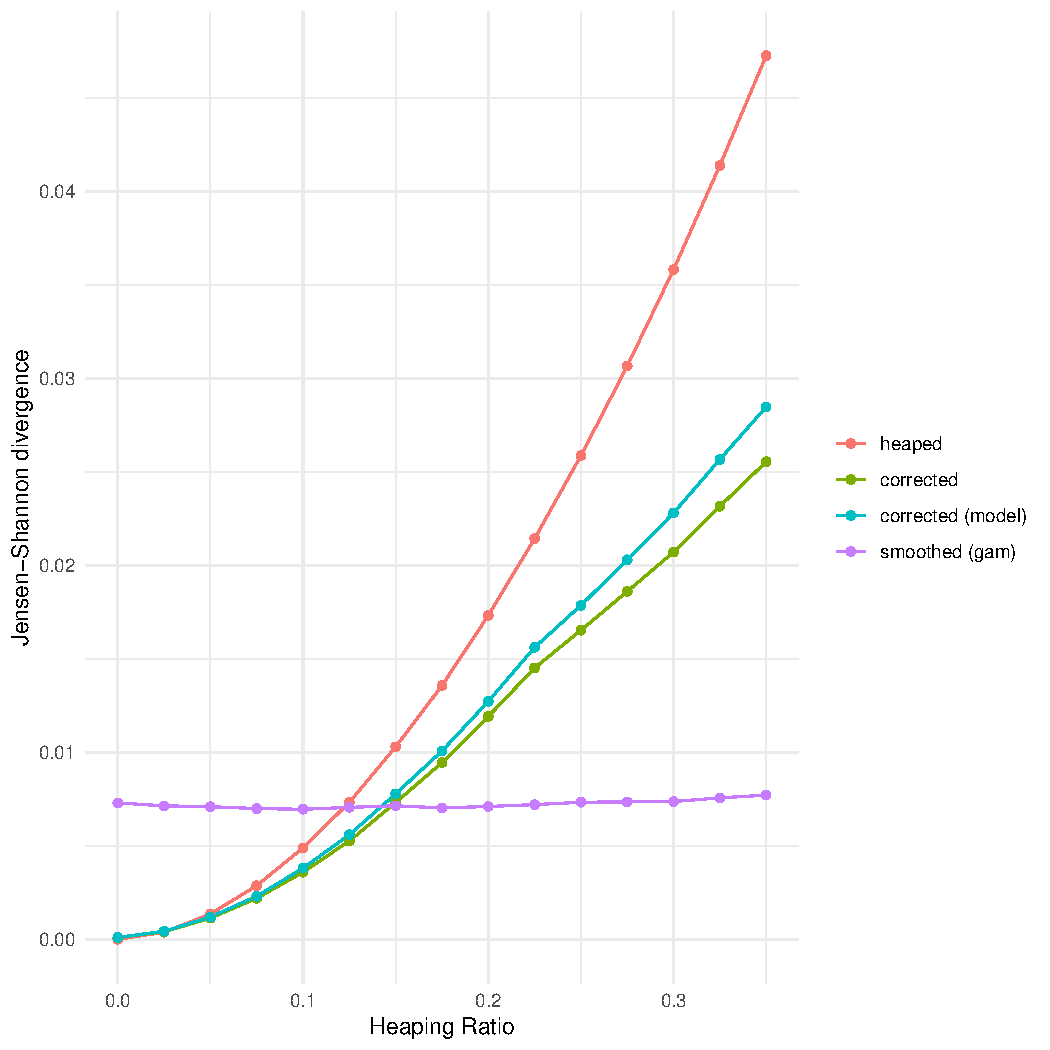
\includegraphics[width=0.8\linewidth]{jsdsim.pdf}
    \caption{Jensen-Shannon divergence from the true age distribution across heaping ratios. Lower values indicate better recovery of the original distribution. The model-based correction achieves the lowest divergence.}
    \label{fig:jsdsim}
\end{figure}

\begin{figure}[!htp]
    \centering
    \includegraphics[width=0.8\linewidth]{mapesim.pdf}
    \caption{Mean Absolute Percentage Error (MAPE) of age-specific counts across heaping ratios. The model-based correction consistently achieves the lowest error rates.}
    \label{fig:mapesim}
\end{figure}

\subsection{Illustrative Examples}

To demonstrate the correction method visually, we generate synthetic age data and introduce artificial heaping. The base population consists of 10,000 ages drawn from a log-normal distribution with parameters $\mu = 2.47$ and $\sigma = 1.65$, rounded to integers and truncated at age 93. This produces a right-skewed age distribution typical of many real-world populations. Heaping is then introduced by duplicating observations at heap ages, creating visible spikes in the distribution.

Figure~\ref{fig:combined5} illustrates the correction of 5-year heaping using the log-normal method (\texttt{method = "lnorm"}). The left panel shows the heaped distribution, where ages ending in 0 or 5 (highlighted in yellow) exhibit substantially higher frequencies than their neighbors. The right panel shows the aggregated distribution after correction. It is important to emphasize that although the bar plots display aggregated frequency distributions, the correction operates at the \emph{individual level}: each corrected observation receives a new age value drawn from the fitted truncated log-normal distribution. The underlying data remains a vector of individual ages that can be linked to other variables and used in subsequent analyses such as regression modeling, record linkage, or machine learning. The artificial peaks have been smoothed, with excess observations redistributed to adjacent ages within $\pm 2$ years of each heap, while the overall shape of the distribution is preserved.

Figure~\ref{fig:combined10} demonstrates the same process for 10-year heaping, again using the log-normal method without model-based adjustment. Here, only ages ending in 0 (highlighted in yellow) are affected. The heaping is more pronounced at each affected age since fewer heap points share the misreported observations. After correction, the peaks at ages 10, 20, 30, etc.\ are reduced to levels consistent with their neighboring ages. The two-stage correction approach for 10-year heaps (using bounds of $\pm 4$ and $\pm 5$ years) distributes the corrected values more broadly than the 5-year case, reflecting the larger rounding error associated with decade-level misreporting. As with the 5-year case, each individual's age is modified separately, preserving the individual-level structure of the data.

For applications where covariate information is available, the model-based correction (\texttt{model} parameter) can further improve results by adjusting the direction of corrections based on predicted ages from a random forest model. This approach is demonstrated in the wage gap analysis (Section~\ref{sec:wagegap}), where the model-based method achieves smaller deviations from the original coefficients compared to the basic correction.

\begin{figure}[!htp]
    \centering
    \begin{subfigure}[b]{0.5\linewidth}
        \centering
        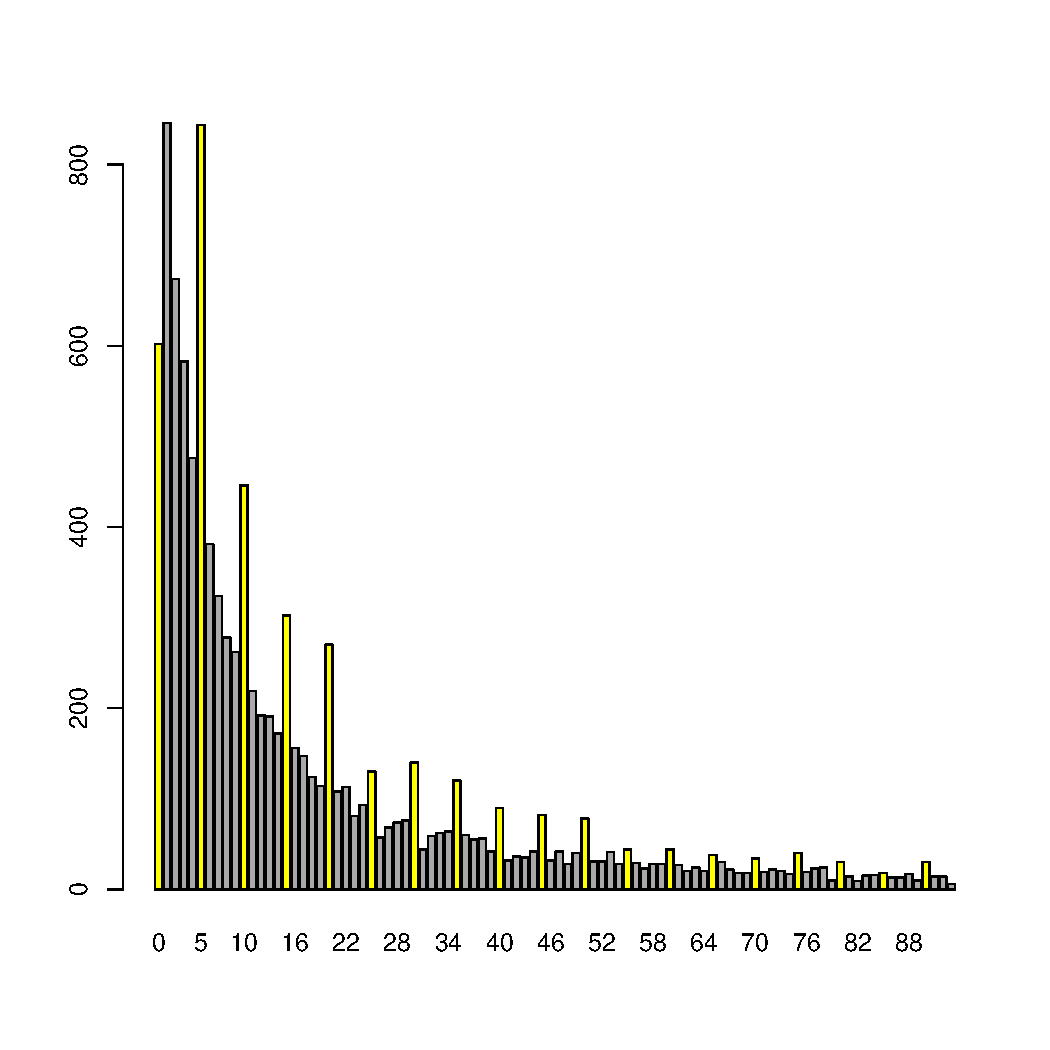
\includegraphics[width=\linewidth]{age5heaps1.pdf}
        \caption{Age distribution with 5-year heaping before correction.}
        \label{fig:age5heaps1}
    \end{subfigure}%
    \begin{subfigure}[b]{0.5\linewidth}
        \centering
        
\includegraphics[width=\linewidth]{age5heaps2.pdf}
        \caption{Age distribution after correction of 5-year heaping.}
        \label{fig:age5heaps2}
    \end{subfigure}
    \caption{Comparison of age distributions before and after correction of 5-year heaping using the proposed individual-level method. Ages ending in 0 or 5 are highlighted in yellow.}
    \label{fig:combined5}
\end{figure}

\begin{figure}[!htp]
    \centering
    \begin{subfigure}[b]{0.5\linewidth}
        \centering
        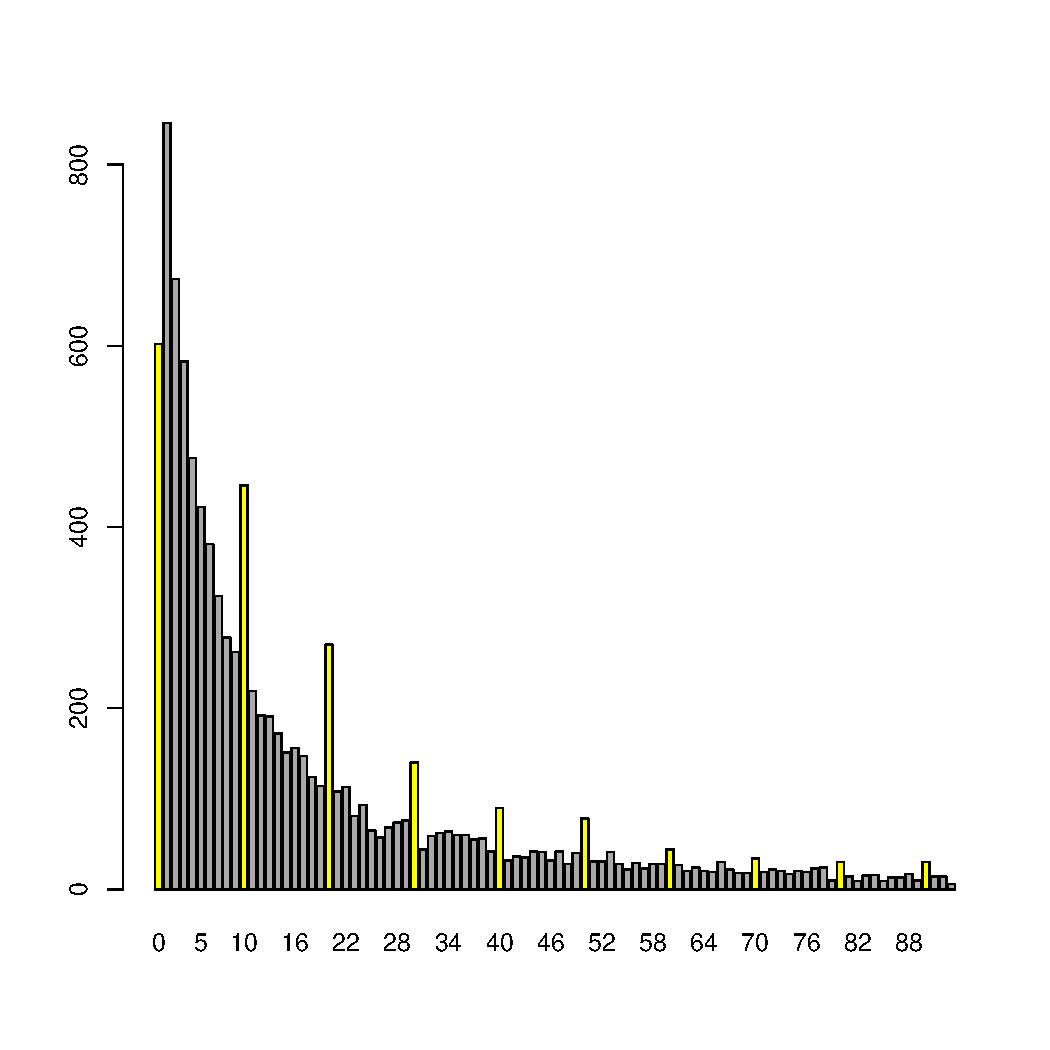
\includegraphics[width=\linewidth]{age10heaps1.pdf}
        \caption{Age distribution with 10-year heaping before correction.}
        \label{fig:age10heaps1}
    \end{subfigure}%
    \begin{subfigure}[b]{0.5\linewidth}
        \centering
        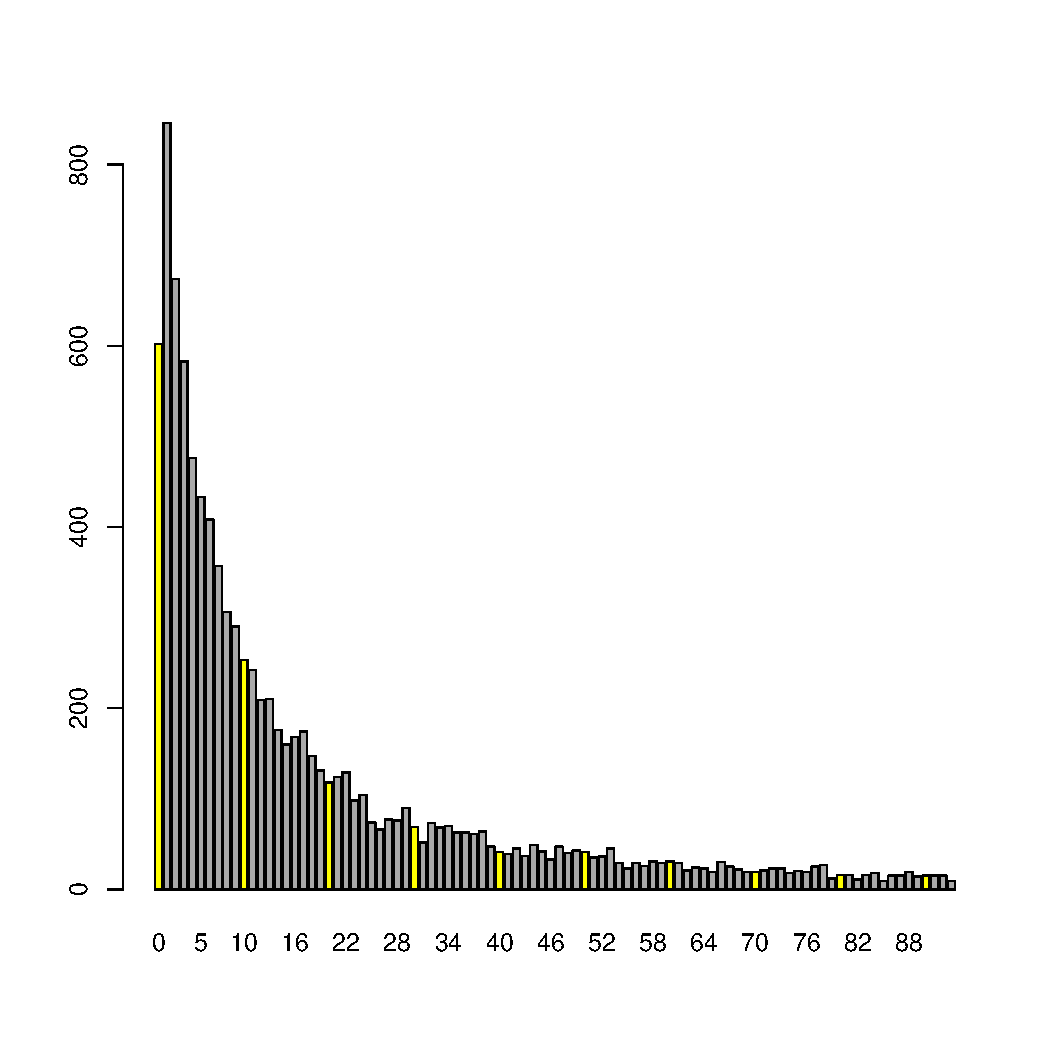
\includegraphics[width=\linewidth]{age10heaps2.pdf}
        \caption{Age distribution after correction of 10-year heaping.}
        \label{fig:age10heaps2}
    \end{subfigure}
    \caption{Comparison of age distributions before and after correction of 10-year heaping using the proposed individual-level method. Ages ending in 0 are highlighted in yellow.}
    \label{fig:combined10}
\end{figure}


\section{Conclusion}

This paper introduced a novel approach for correcting heaping at the individual level, addressing a gap in the demographic and statistical literature where traditional methods focus primarily on smoothing aggregated statistics. While established techniques such as the Carrier-Farrag \citep{carrier1959}, Arriaga \citep{arriaga1968}, Karup-King-Newton \citep{karup1903}, and United Nations \citep{un1956} formulas effectively smooth population distributions, they do not preserve individual-level data integrity, which is essential for regression modeling, longitudinal studies, and machine learning applications.

The proposed method identifies heaped values by comparing observed frequencies at heaping points (ages ending in 0 or 5) with the mean frequency of adjacent ages. A calculated proportion of observations at each heaping point is then redistributed using draws from truncated distributions---log-normal, normal, uniform, or kernel density estimates---fitted to the underlying data. This stochastic approach ensures that corrected values remain plausible while eliminating artificial peaks in the distribution.

The application to wage gap analysis using the Blinder-Oaxaca decomposition demonstrated the practical importance of individual-level correction. As shown in Table~\ref{tab:twofold}, the model-based correction approach achieved the smallest deviation from the original (unheaped) coefficients, with differences of only 1.93\% and 1.90\% for Groups A and B, respectively. This compares favorably to the naive correction without modeling, which showed larger deviations of 10.29\% and 5.45\%. These results confirm that preserving the distributional characteristics of the data through model-based correction leads to more accurate downstream analyses.

Several advantages of the individual-level approach were identified: (1) preservation of data granularity for detailed analyses, (2) flexibility to use the same corrected dataset across multiple studies, (3) improved accuracy in regression models and predictive algorithms, (4) compatibility with longitudinal study designs, and (5) better detection of anomalies that might be masked by aggregated smoothing.

The method has some limitations. First, it assumes that heaping is the result of misreporting rather than systematic underreporting; if age/sex-specific underreporting exists, the correction may inappropriately redistribute observations \citep{preston1999}. Second, the quality of the correction depends on the appropriateness of the fitted distribution; for highly skewed or multimodal data, the log-normal or kernel methods are preferred over the normal distribution. Third, the stochastic nature of the correction means that results vary across runs unless a random seed is specified, though this can be advantageous for multiple imputation frameworks.

Future work could extend the method in several directions. Integration with multiple imputation frameworks would allow proper uncertainty quantification across analyses. The approach could be generalized to other types of heaping beyond age data, including income, body weight, and time duration. Additionally, Bayesian methods could be incorporated to provide posterior distributions of corrected values rather than point estimates.

The proposed methods are implemented in the R package \texttt{heaping}, which provides the functions \texttt{correctHeaps()} for systematic heaping correction and \texttt{correctSingleHeap()} for targeted correction at specific values. The package supports multiple distribution methods, reproducible results through seed specification, and diagnostic output for assessing correction quality. In addition to correction functions, the package implements all major heaping indices (Whipple, Myers, Bachi, Noumbissi, Spoorenberg, Coale-Li, Jdanov, Kannisto) with support for sampling weights, enabling comprehensive heaping diagnostics for survey data. The software is available to facilitate adoption of individual-level heaping correction in demographic research, survey analysis, and data science applications.


%% ============================================================================
%% DATA AVAILABILITY STATEMENT (required by JSSAM)
%% ============================================================================

\section*{Data Availability Statement}

The datasets used in this study are publicly available. The \texttt{chicago} dataset is available in the R package \texttt{oaxaca} on CRAN. Synthetic data for the simulation studies were generated using the parameters described in Section 3. The R package \texttt{heaping} implementing the proposed methods is available on GitHub at \url{https://github.com/matthias-da/heaping} and is already submitted to CRAN. Complete replication code is available upon request. %% [Author contact details removed for blind review]

%% ============================================================================
%% DECLARATIONS
%% ============================================================================

\section*{Declarations}

\begin{itemize}
\item \textbf{Funding}: Not applicable.
\item \textbf{Conflict of interest}: The authors declare no conflict of interest. %% [Anonymized for blind review]
\end{itemize}

%% ============================================================================
%% REFERENCES (ASA style via natbib/apalike)
%% ============================================================================

\bibliography{sn-bibliography}


\end{document}
